\chapter{Asymptotic normality of estimating-equation M-estimators.}
\begin{figure}[H]
\centering
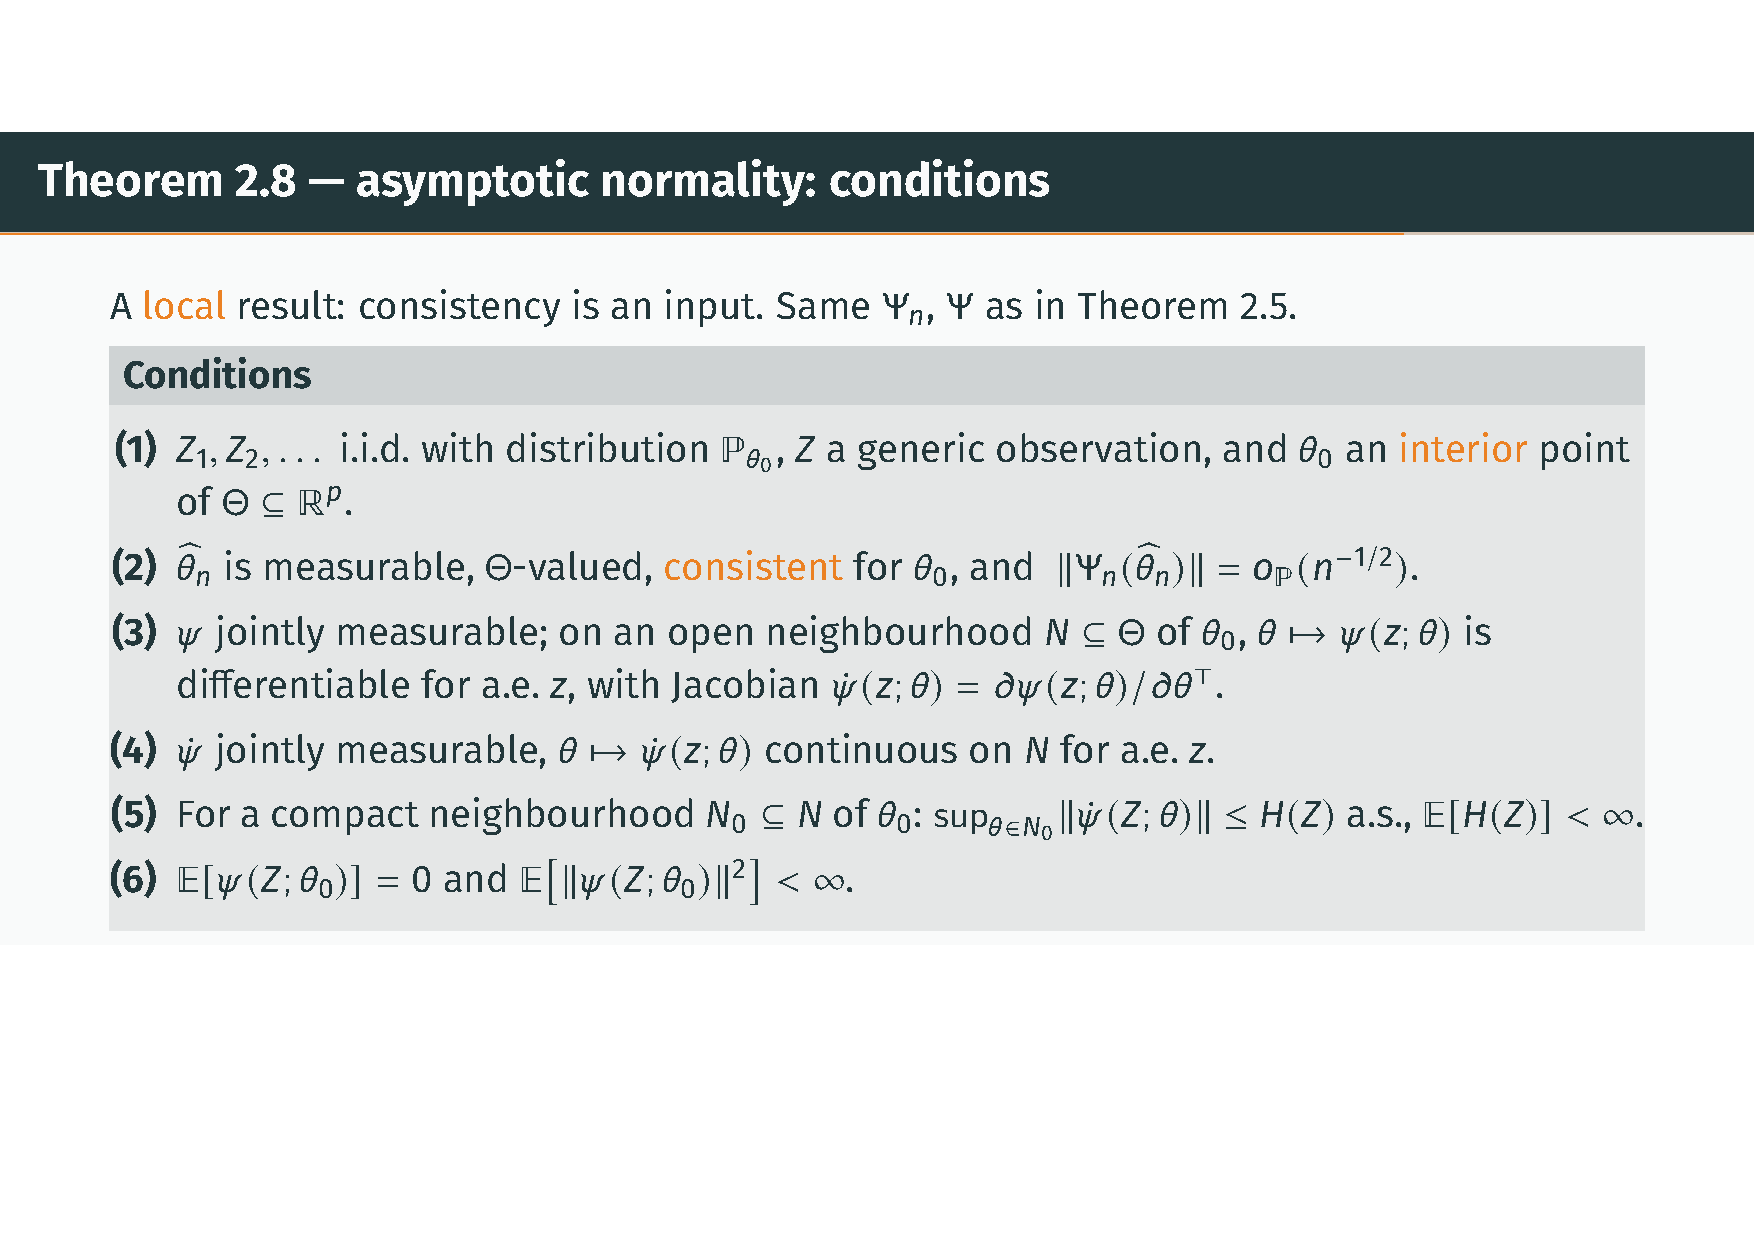
\includegraphics[width=\textwidth]{figures/Asymptotic-1.pdf}
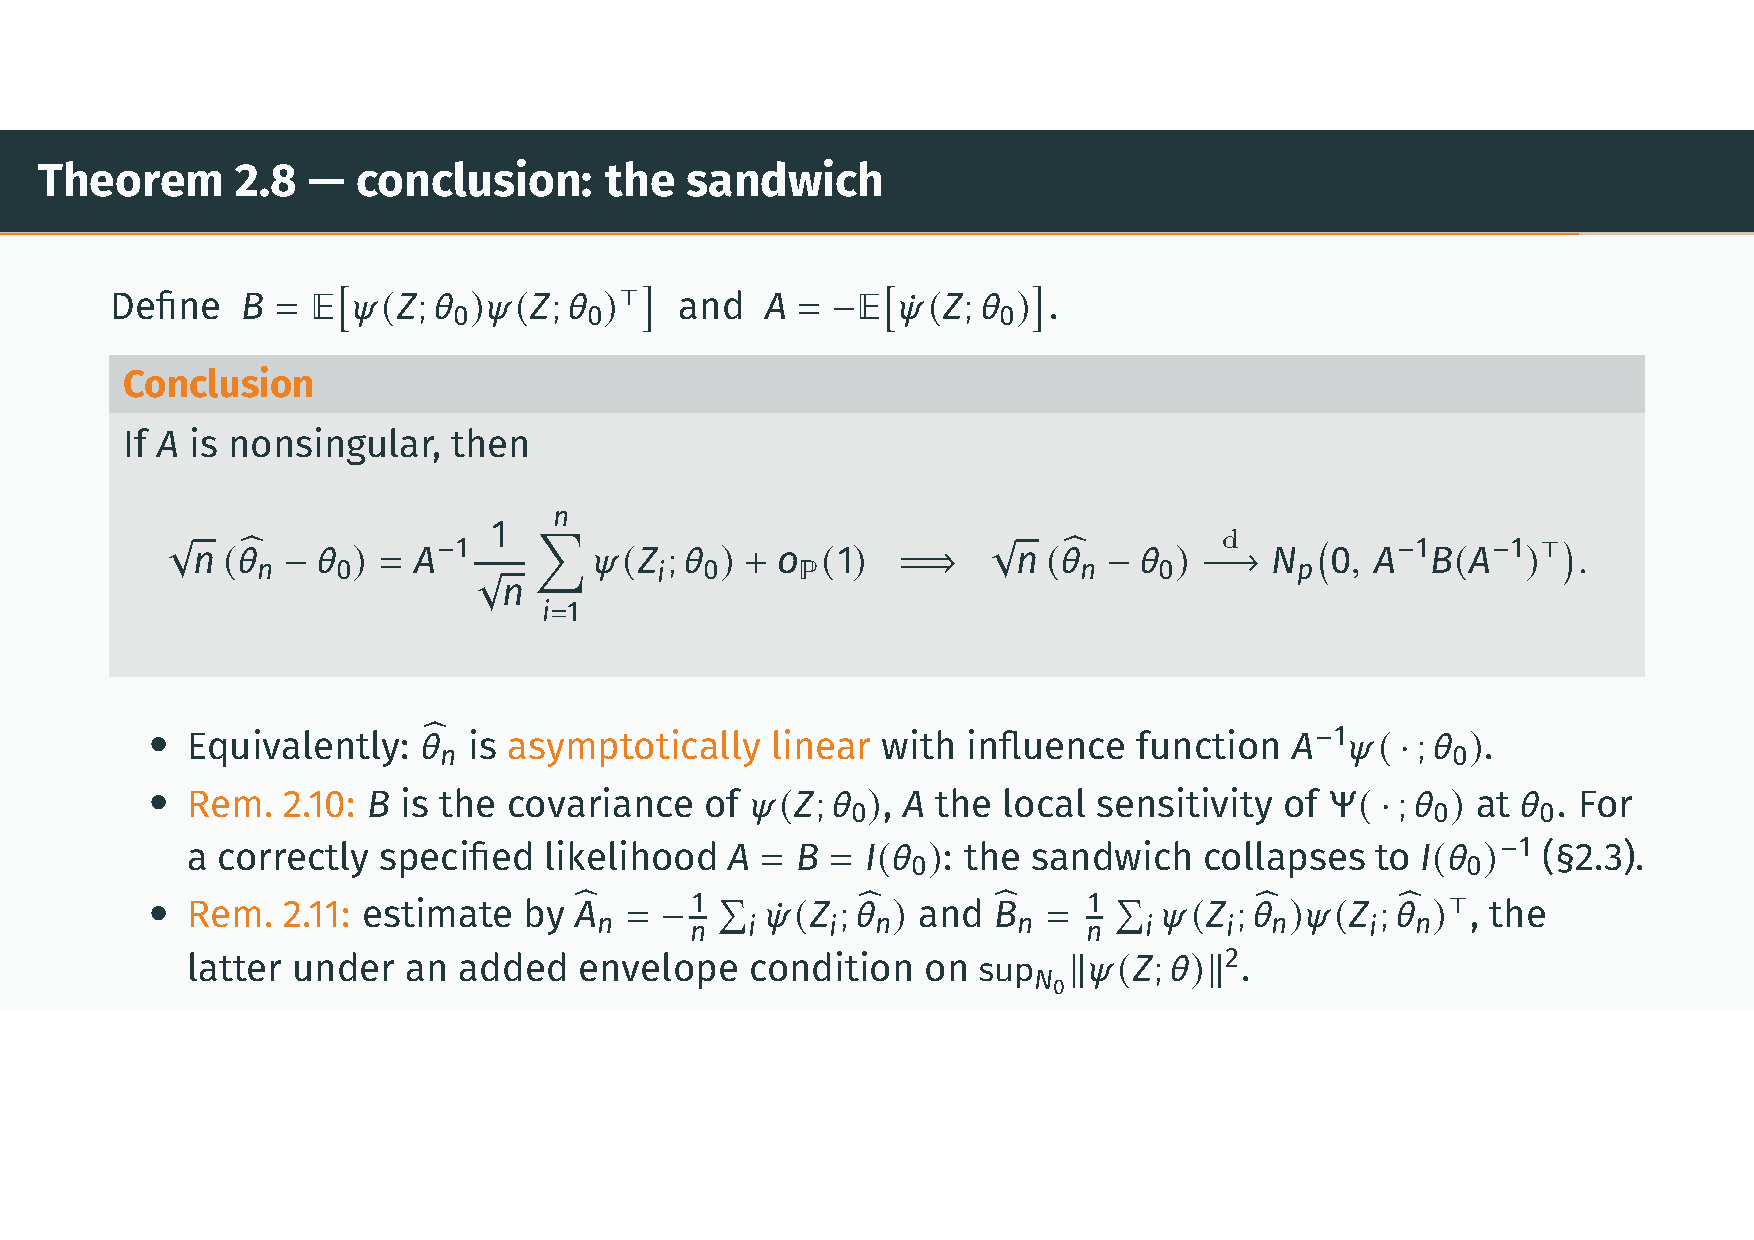
\includegraphics[width=\textwidth]{figures/Asymptotic-2.pdf}
\end{figure}
\noindent\textbf{Comments}
\global\def\lastproofcolor{theorembordercolor} % needed since no theorem is used here
\begin{proof}
  Since \textbf{(3)} and \textbf{(4)} are both almost sure events, there exists an event $\Omega_1$,
  where, for all $i\ge 1$ the map $\theta \mapsto \psi(Z_i;\theta)$ is differentiable on $N$ with
  derivative $\dot\psi(Z_i;\theta)$ continuous on $N$.

  \begin{description}
    \item[1) Localization] 
  \end{description}
  Since $N_0$ is a neighborhood of $\theta_0$, there exists a radius $\eta >0$ such that
  $\overline{B}(\theta_0, \eta)=\{ \theta \in \Theta :  \| \theta - \theta_0 \| \le \eta \} \subseteq  N_0$. By the consistency assumption,
  \textbf{(2)}, 
  \[ 
    \P(\| \what{\theta}_n -\theta_0 \| \le \eta) \to  1
  .\]


  \begin{description}
    \item[2) Taylor expansion along the segment to $\what{\theta}_n$] 
  \end{description}
  On $E_n = \Omega_1 \cap  \overline{B}(\theta_0,\eta)$ the line segment between $\theta_0$ and
  $\what{\theta}_n$ is contained in $N$. Applying the fundamental theorem of calculus along this
  line segment gives:
  \begin{equation} 
    \Psi_n(\what{\theta}_n) = \Psi_n(\theta_0) + \overline{K}_n (\what{\theta}_n - \theta_0), \quad 
    \overline{K}_n = \int_{0}^{1} \dot\Psi_n(\theta_0 + t(\what{\theta}_n - \theta_0)  \d t, 
    \;\; \dot\Psi_n = \frac{1}{n} \sum_{i=1}^{n} \dot\psi(Z_i;\theta)
    \label{eq:disp2-fund-thrm-cal}
  ,\end{equation}
  On $E_n$. Outside $E_n$ define $\overline{K}$ as the zero matrix.
  \textcolor{gray}{
    Note that \Cref{eq:disp2-fund-thrm-cal} is
    the integral form of the first order Taylor expansion of $\Psi_n$ along its line segment from
  $\theta_0$ to $\theta_n$, with $\overline{K}$ being the average Jacobian along this segment.}

  \begin{description}
    \item[3) The averaged Jacobian converges to $-A$] 
  \end{description}
  Let $\dot\Psi(\theta;\theta_0) = \E[\dot\psi(Z;\theta)]$, well-defined by \textbf{(5)}. Note that
  the regularity \textbf{(4)} and envelope \textbf{(5)} assumptions gives a uniform law of large
  numbers: 
  \begin{equation} 
    \sup_{\theta \in N_0} \| \dot\Psi_n(\theta) - \dot\Psi(\theta; \theta_0) \| \xrightarrow[n \to
    \infty ]{a.s.} 0
    \label{eq:disp2-ulln}
  ,\end{equation}
  in particular also in probability. Furthermore, dominated convergence implies that $\dot\psi(\cdot
  ;\theta_0)$ is continuous at $\theta_0$.

  On $E_n$, the segment from $\theta_0$ to $\what{\theta}_n$ lies in $N_0$, so the triangle
  inequality applied inside the integral defining $\overline{K}_n$ gives  
  \begin{equation} 
  \| \overline{K}_n - \dot\Psi(\theta_0;\theta_0) \| \le  \sup_{\theta \in N_0} \|
  \dot\Psi_n(\theta) - \dot\Psi(\theta;\theta_0) \| + \sup_{t \in [0,1]} \| \dot\Psi (\theta_0 +
  t(\what{\theta}_n - \theta_0);\theta_0) - \dot\Psi(\theta_0; \theta_0)\|
  \label{eq:disp2-triangle-ineq}
  .\end{equation}
  The fist term converges to 0 a.s. by \Cref{eq:disp2-ulln}. For the second term, fix $\epsilon >0$.
  By continuity of $\dot\Psi(\cdot ;\theta_0)$ at $\theta_0$:
  \[ 
    \exists \delta \in (0, \eta] 
    \quad  \text{s.t. }\quad
    \| \theta - \theta_0 \| < \delta 
    \quad \implies  \quad 
    \| \dot\Psi(\theta;\theta_0) - \dot\Psi(\theta_0; \theta_0) \| < \epsilon
  .\]
  For all $t \in [0,1]$, the point $\theta_0 + t(\what{\theta}_n- \theta_0)$ lies within $\|
  \what{\theta}_n - \theta_0 \|$ of $\theta_0$. Therefore, on $M_n = \{ \| \what{\theta}_n  -
  \theta_0\| <\delta\}$, the second term is below $\epsilon$. Moreover, by consistency the events
  $M_n$ tend to 1 in probability. Thus, the second term in \Cref{eq:disp2-triangle-ineq} is $o_{\P}
  (1)$.

  Since $\P(\Omega_1) = 1$ and $\P(M_n) \xrightarrow[]{} 1$, the triangle inequality in
  \Cref{eq:disp2-triangle-ineq} holds with probability tending to 1, and since we have just shown
  the thow terms on the right hand side converge to 0 in probability, we must have:
  \[ 
  \overline{K}_n \xrightarrow[n \to \infty ]{\P} \dot \Psi(\theta_0;\theta_0) =
  \E[\dot\psi(Z;\theta_0)] =- A
  .\]

  \begin{description}
    \item[4) Solving for $\sqrt{n}(\what{\theta}_n - \theta_0)$] 
  \end{description}
  Let $D_n$ be the event that $\overline{K}_n$ is nonsingular. Since $\overline{K}_n$ equals the
  zero matrix outside $E_n$ and the zero matrix is singular, $D_n \subseteq  E_n$. Moreover,
  \Cref{eq:disp2-fund-thrm-cal} holds on $D_n$. Since $\overline{K}_n \xrightarrow[]{\P} -A$ and $A$
  is nonsingular, $\P(D_n) \to 1$. 

  Define $\tilde{K}_n^{-1}= \overline{K}^{-1}_n$ on $D_n$ and $\tilde{K}_n^{-1} = 0$ on $D_n^{c}$.
  By continuity of the inverse map on the set of nonsingular matrices, $\tilde{K}_n^{-1}
  \xrightarrow[]{\P} -A^{-1}$.

  Rearrange \Cref{eq:disp2-fund-thrm-cal} to get:
  \[ 
  \sqrt{n}(\what{\theta}_n - \theta_0) =
  -\overline{K}_n^{-1}\sqrt{n}\Psi_n(\theta_0) 
  + \overline{K}^{-1}_n \sqrt{n}\Psi_n(\what{\theta}_n)
  ,\]
  on $D_n$. But $\P(D_n) \to 1$ so
  \[ 
  \sqrt{n}(\what{\theta}_n - \theta_0) =
  -\tilde{K}_n^{-1}\sqrt{n}\Psi_n(\theta_0) 
  + \tilde{K}^{-1}_n \sqrt{n}\Psi_n(\what{\theta}_n) + o_{\P}(1)
  .\]
  Since $\tilde{K}_n^{-1} \xrightarrow[]{\P} -A^{-1}$ and $\sqrt{n}\Psi_n(\what{\theta}_n) =
  o_{\P}(1)$ (by \textbf{(2)}), it follows that:
  \[ 
  \sqrt{n}(\what{\theta}_n - \theta_0) = A^{-1}\sqrt{n}\Psi_n(\theta_0) + o_{\P}(1)
  = A^{-1}\frac{1}{\sqrt{n}} \sum_{i=1}^{n} \psi(Z_i;\theta_0)+ o_{\P}(1)
  .\]
  By \textbf{(6)} we can apply the multivariate central limit theorem to get:
  \[ 
    \frac{1}{\sqrt{n}} \sum_{i=1}^{n} \psi(Z_i;\theta_0) \xrightarrow[n \to \infty ]{d} N(0, B)
  .\]
  The claimed asymptotic normality follows by Slutsky's Theorem.
  \qed
\end{proof}



\section{Relevant results}
\begin{theorem*}[(Slutsky's theorem (ChatGPT))]
Let $(X_n)_{n\in\N}$ and $(Y_n)_{n\in\N}$ be random vectors such that
\[
  X_n \xrightarrow[n\to \infty ]{d} X
\qquad \text{and} \qquad
Y_n \xrightarrow[n\to \infty ]{\P} c,
\]
where $X$ is a random vector and $c$ is a constant vector. Then, for any continuous function
$g:\R^{k}\times\R^{m}\to\R^{r}$,
\[
  g(X_n,Y_n)\xrightarrow[n\to \infty ]{d}g(X,c).
\]
\end{theorem*}
\begin{theorem*}[(Multivariate central limit theorem (from ChatGPT))]
Let $(X_n)_{n\in\N}$ be a sequence of i.i.d. random vectors in $\R^d$ satisfying $\E[\|X_1\|^2]<\infty.$ Define
\[
\mu=\E[X_1],
\qquad
\Sigma=\operatorname{Cov}(X_1).
\]
Then
\[
\sqrt{n}\left(\frac{1}{n}\sum_{i=1}^n X_i-\mu\right)
\xrightarrow{d} N_d(0,\Sigma),
.\]
\end{theorem*}

\begin{remark*}[2.10 (Interpretation of $A$ and $B$)]
  The matrix $B = \E[\psi(Z;\theta_0)\psi(Z;\theta_0)^{\top }]$  is the covariance matrix of the
  estimating function at $\theta_0$, since $\E[\psi(Z;\theta_0)] = 0$. The matrix $A =
  -\E[\dot\psi(Z;\theta_0)]$ measures the local sensitivity of the population estimating equation
  $\Psi(\theta;\theta_0)$ at $\theta_0$. The asymptotic covariance matrix $A^{-1}B(A^{-1})^{\top }$
  is the \textbf{sandwich covariance matrix}.

  For likelihood scores under correct specification and standard regularity conditions, the
  information identity gives $A = B = I(\theta_0)$, where $I(\theta_0)$ is the Fisher information pr
  observation, so the sandwich reduces to $I(\theta_0)^{-1}$, see section 2.3 in the notes.
\end{remark*}


\begin{remark*}[2.9 (Existance of local roots)]

  \fxnote{Figure out if this is relevant}
\end{remark*}


\section{Applications}
\label{sec:}

